\documentclass[paper=a4, fontsize=12pt]{scrartcl} % A4 paper and 11pt font size
\usepackage[margin=1in]{geometry}  

\usepackage[T1]{fontenc} % Use 8-bit encoding that has 256 glyphs
\usepackage{fourier} % Use the Adobe Utopia font for the document - comment this line to return to the LaTeX default
\usepackage[english]{babel} % English language/hyphenation
\usepackage{amsmath,amsfonts,amsthm} % Math packages
\usepackage{enumerate}
\usepackage{graphicx}
\usepackage{caption}

\usepackage{sectsty} % Allows customizing section commands
\allsectionsfont{\raggedright \normalfont\scshape} % Make all sections centered, the default font and small caps

\usepackage{fancyhdr} % Custom headers and footers
\pagestyle{fancyplain} % Makes all pages in the document conform to the custom headers and footers
\fancyhead[R]{\emph{Scaling/Approximation - Chapter 11 and 14}} % No page header - if you want one, create it in the same way as the footers below
\fancyfoot[L]{} % Empty left footer
\fancyfoot[C]{} % Empty center footer
\fancyfoot[R]{\thepage} % Page numbering for right footer
\renewcommand{\headrulewidth}{0pt} % Remove header underlines
\renewcommand{\footrulewidth}{0pt} % Remove footer underlines
\setlength{\headheight}{13.6pt} % Customize the height of the header

\numberwithin{equation}{section} % Number equations within sections (i.e. 1.1, 1.2, 2.1, 2.2 instead of 1, 2, 3, 4)
\numberwithin{figure}{section} % Number figures within sections (i.e. 1.1, 1.2, 2.1, 2.2 instead of 1, 2, 3, 4)
\numberwithin{table}{section} % Number tables within sections (i.e. 1.1, 1.2, 2.1, 2.2 instead of 1, 2, 3, 4)

%----------------------------------------------------------------------------------------
%	TITLE SECTION
%----------------------------------------------------------------------------------------

\newcommand{\horrule}[1]{\rule{\linewidth}{#1}} % Create horizontal rule command with 1 argument of height

\author{\vspace{-5ex}}
\date{\vspace{-10ex}}
\title{	
\normalfont \normalsize 
\textsc{Chem-Eng 321: Fluid Mechanics} \\ [10pt] % Your university, school and/or department name(s)
\horrule{0.5pt} \\[0.2cm] % Thin top horizontal rule
\huge Scaling/Approximation \\ (Denn Chapter 11 and 14) \\ % The assignment title
\horrule{2pt} \\[0.2cm] % Thick bottom horizontal rule
}


\begin{document}

\maketitle % Print the title

\thispagestyle{empty}

\section*{Learning Objectives}

\begin{enumerate}
\item Scale conservation equations. Analyze scaled equation. 
\item Solve and analyze inviscid flow problems using stream functions and potential flows.

\end{enumerate}

\section*{Motivation}

Throughout this course we've encountered situations where an approximation has simplified our problem solving and analysis. Examples?

As a corollary, we should be able to rewrite our conservation equations (e.g. Navier-Stokes) in a form approximate to the situation. Hopefully, a solution to the approximate equations is an approximate solution. 

\section*{Rewriting Navier-Stokes Equations (Chapter 11)}

Consider Steady Navier-Stokes Equation:

\vspace{2ex} \begin{equation*}
\rho \underline{\mathbf{v}} \cdot \underline{\nabla}  \underline{\mathbf{v}} = -\underline{\nabla} \mathcal{P}+\eta \nabla^2 \underline{\mathbf{v}} 
\end{equation*}

And a general flow past an object problem:

\hspace*{6cm} 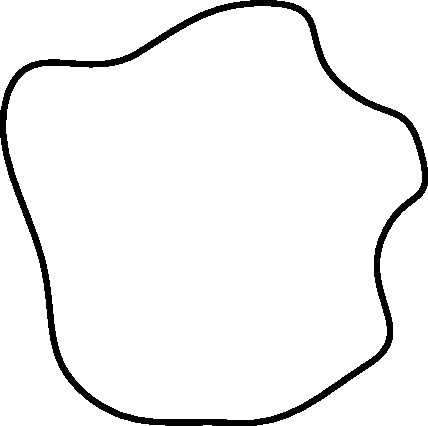
\includegraphics[scale=0.5]{drawing.pdf}

 Re-write the Navier Stokes problems in terms of the "Scaled Variables"
  \begin{itemize}
  \item 
  \item 
\end{itemize}
\newpage

\subsection*{Scaling Our Variables}
We can rescale our variables appropriately: 

Scaled velocity $\widetilde{\underline{\mathbf{v}}}=\widetilde{\mathbf{v}}/V$

\vspace{5ex}Scaled coordinate $\widetilde{\underline{\mathbf{x}}}=\widetilde{\mathbf{x}}/L$

\vspace{5ex} What about pressure? $\widetilde{\underline{\mathcal{P}}}=\widetilde{\mathcal{P}}/\Pi$


\vspace{5ex} Typical Inertial Term
\vspace{2ex} \begin{equation*}
\rho v_x \frac{\partial v_y}{\partial x} \hspace{5ex} v_x=\widetilde{v_x}V
\hspace{5ex} v_y=\widetilde{v_y}V
\hspace{5ex} x=\widetilde{x}L
\end{equation*}
Plug in...


\vspace{2cm}  As a result we can rewrite the left side of N-S as

\vspace{2ex} \begin{equation*}
\hspace{-8cm} \rho \underline{\mathbf{v}} \cdot \underline{\nabla}  \underline{\mathbf{v}} \Rightarrow
\end{equation*}

\vspace{2cm}  Now for the viscous term:
\vspace{2ex} \begin{equation*}
\eta \frac{\partial^2 v_x}{\partial y^2} \hspace{5ex} v_x=\widetilde{v_x}V
\hspace{5ex} y=\widetilde{y}L
\end{equation*}

Plug in...

\vspace{2cm} Viscous terms in general: $\eta \nabla^2 \underline{\mathbf{v}} \Rightarrow$


\vspace{1cm}  And pressure:
\vspace{2ex} \begin{equation*}
\frac{\partial \mathcal{P}}{\partial x} \hspace{5ex} \mathcal{P}=\widetilde{\mathcal{P}}\Pi
\hspace{5ex} x=\widetilde{x}L
\end{equation*}
Plug in...

\newpage

Rewrite our Navier-Stokes Equation:


\vspace{2cm} If variables are properly scaled, then all dimensionless terms are $O(1)$ quantities. 

\vspace{1cm} $\Rightarrow$

\vspace{1cm} In particular,

\vspace{1cm} This provides basis for \underline{approximations}.

\vspace{1cm} When Re $>>$ 1, expect 

\vspace{0.5cm} $\Rightarrow$ Approximate by neglecting

\vspace{0.5cm} $\Rightarrow$ \underline{Inviscid flow}

\vspace{1cm} When Re $<<$ 1, expect 

\vspace{0.5cm} $\Rightarrow$ Approximate by neglecting

\vspace{0.5cm} $\Rightarrow$ \underline{Creeping flow}

\vspace{1cm} What about pressure?

\vspace{2cm} \hspace{1cm} When inertial terms dominate (high Re), pressure balances with

 \vspace{1cm} \hspace{6cm} $\Rightarrow \Pi =$

\vspace{1cm} \hspace{1cm} When viscous terms dominate (low Re), pressure balances with

 \vspace{1cm} \hspace{6cm} $\Rightarrow \Pi = $


\newpage

Thus, for High Reynold's Number (inertial dominated) flow, we can write:

\vspace{2ex} \begin{equation*}
 \hspace{-6cm}  \underline{\widetilde{\mathbf{v}}} \cdot \underline{\widetilde{\nabla}}  \underline{\widetilde{\mathbf{v}}} = -\underline{\widetilde{\nabla}} \mathcal{\widetilde{P}}+\frac{1}{\text{Re}} \widetilde{\nabla}^2 \underline{\widetilde{\mathbf{v}}} \Rightarrow 
\end{equation*}

\vspace{2ex} Thus, for Low Reynold's Number (viscous dominated) flow, we can write:

\vspace{2ex} \begin{equation*}
 \hspace{-6cm}  \text{Re} (\underline{\widetilde{\mathbf{v}}} \cdot \underline{\widetilde{\nabla}}  \underline{\widetilde{\mathbf{v}}}) = -  \underline{\widetilde{\nabla}} \mathcal{\widetilde{P}}+ \widetilde{\nabla}^2 \underline{\widetilde{\mathbf{v}}} \Rightarrow 
\end{equation*}

\vspace{2ex}  \textbf{We hope that solutions of the approximation equations is an approximate solution to the problem. (Denn 11.6)}

\vspace{1cm} \hspace*{2cm} \begin{tabular*}{11cm}{c @{\extracolsep{\fill}} c}
\underline{High Re} & \underline{Low Re} \\

\end{tabular*}

\newpage

\section*{High Reynold's Number (Inviscid Flow)}
\vspace{2ex} \begin{equation*}
\hspace*{-8cm} \text{Re}=\frac{Dv\rho}{\eta} \Rightarrow
\end{equation*}

However, we face some challenges with this equation. Need to define some other concepts before solving inviscid flow solutions. In particular, we seek \underline{Potential Flows} (Denn Chp. 14).

\section*{Stream Function (Chapter 14)}
Useful in 2-D flow (e.g. $v_x(x,y)$,$v_y(x,y)$, and $v_z=0$)

Case without a Stream function:
\vspace{0ex} \begin{align*}
\hspace*{-6cm} v_x(x,y) & \\
\hspace*{-6cm}  v_y(x,y) & \\
\hspace*{-6cm}  \mathcal{P}(x,y) &
\end{align*}

Define Stream Function, $\Psi(x,y)$:

\vspace{-7ex} \begin{align*}
 v_x(x,y) &= 
\\ \vspace{5ex}  v_y(x,y) &= 
\end{align*}

Plug into continuity: 

\vspace{2ex} \begin{equation*}
\hspace*{-8cm} \frac{\partial v_x}{\partial x} +  \frac{\partial v_y}{\partial y} =
\end{equation*}

\vspace{2ex} Now we have
\vspace{-2ex} \begin{align*}
\hspace*{-4cm} \Psi(x,y) & \\
\hspace*{-4cm}  \mathcal{P}(x,y) & 
\end{align*}

\vspace{2ex}  In steady flow, the stream function doesn't change along the streamline. We can prove this by taking the substantial derivative:

\vspace{2ex} \begin{equation*}
\hspace*{-8cm} \frac{D \Psi}{D t}= v_x \frac{\partial \Psi}{\partial x} + v_y \frac{\partial \Psi}{\partial y} =
\end{equation*}

\vspace{2cm}  For cylindrical coordinates:

\vspace{2ex} \begin{equation*}
\hspace*{-8cm} v_r= \hspace*{4cm} v_{\theta} =
\end{equation*}

\end{document}

\end{document}